\documentclass[border=1pt, 12pt, tikz]{standalone}

\newcommand\wideOne{3cm}
\newcommand\wideTwo{4cm}
\newcommand\wideThree{2.7cm}
\newcommand\wideFour{3cm}
\newcommand\distOne{2cm}
\newcommand\distTwo{1cm}

\begin{document}
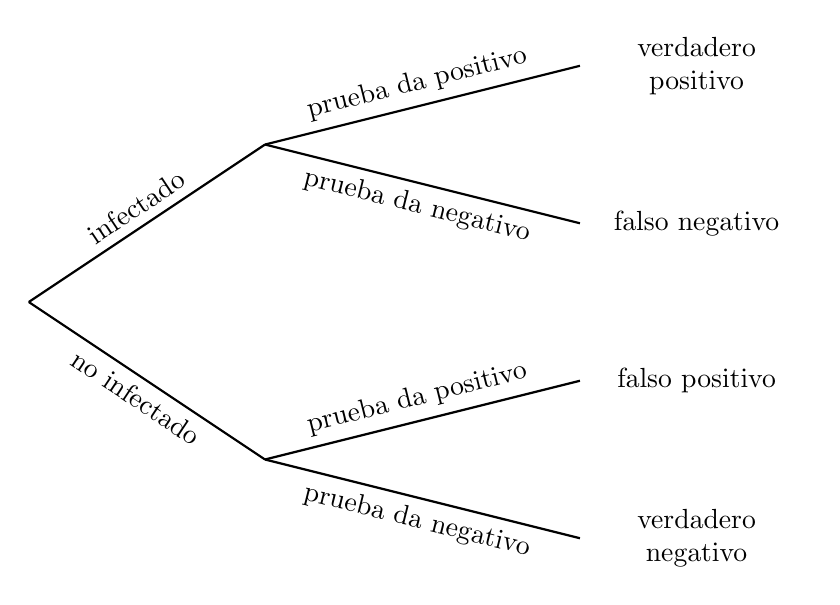
\begin{tikzpicture}[scale=1]

% 1st level
\draw[thick]%
   (0,0) 
   -- node[above, sloped, align=center]
      {infectado} 
   (\wideOne,\distOne);
\draw[thick] 
   (0,0) 
   -- node[below, sloped, align=center]
      {no infectado} 
   (\wideOne,-\distOne);

% 2nd, 3rd and 4th Level
\draw[thick] 
   (\wideOne,\distOne)
   -- node[above, align=center, sloped]
      {prueba da positivo}
   ++ (\wideTwo,\distTwo) 
      node[right, align=center, text width=\wideThree]
      {verdadero positivo}
   ; 
\draw[thick] 
   (\wideOne,\distOne) 
   -- node[below, align=center, sloped]
      {prueba da negativo}
   ++ (\wideTwo,-\distTwo) 
      node[right, align=center, text width=\wideThree]
      {falso negativo}
   ;
\draw[thick] 
   (\wideOne,-\distOne) 
   -- node[above, align=center, sloped]
      {prueba da positivo}
   ++ (\wideTwo,\distTwo) 
      node[right, align=center, text width=\wideThree]
      {falso positivo}
   ;  
\draw[thick] 
   (\wideOne,-\distOne)
   -- node[below, align=center, sloped]
      {prueba da negativo}
   ++ (\wideTwo,-\distTwo) 
      node[right, align=center, text width=\wideThree]
      {verdadero negativo}
   ; 
\end{tikzpicture}
\end{document}
